\section{Example: Multivariable Linear Regression}
A linear regression model for 2 features:
\begin{align*}
 y &= w_1\cdot x_1 + w_2\cdot x_2 + b \\
   &= \vec{w}\cdot\vec{x} + b
\end{align*}
$w_1$,$w_2$ control the slopes of this plane, $b$ translates it up and down. $\vec{x}$ is for one sample. Two or more samples are represented as a matrix:
\begin{align}
[y1, y2] = 
  [w1, w2]\cdot{}
  \begin{bmatrix}
  x_1 & x_1\\
  x_2 & x_2 
  \end{bmatrix}
 +  b
\end{align}
$y_i$ is the result for each sample (columns in the matrix).

We need to do forward and backward propagation.

The same than for a line (figure \ref{fig:line}) by tuning $W$ and $b$  we can find the best fit. Without $b$ the line has to go through the origin. 

The sign of $W$ reflects the line over $y$ axis, and the magnitude controls the slope. Also $b$ translates over $x$.

\begin{figure}[h]
 \centering
 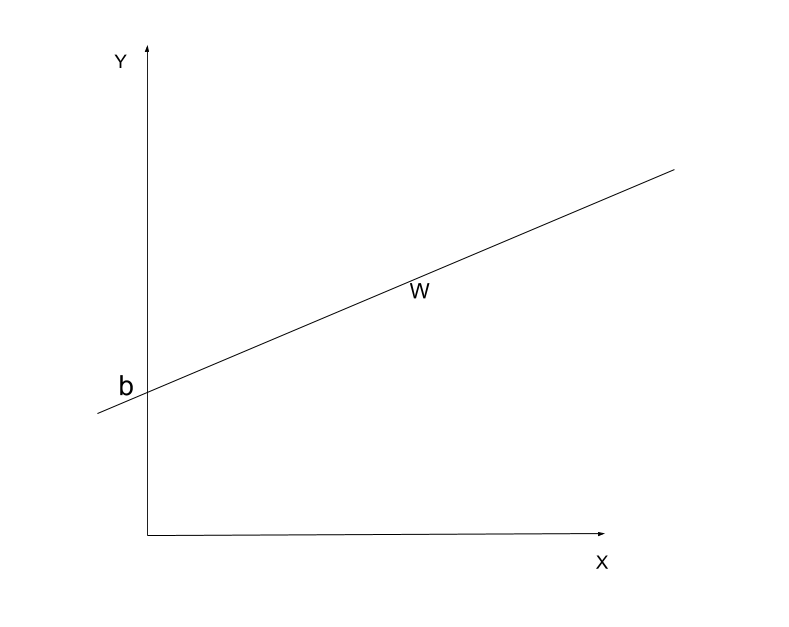
\includegraphics[width=0.9\textwidth]{line_plot.png}
  \caption{Line plot} \label{fig:line}
\end{figure}


\subsection{Forward Propagation}
The Loss $= Loss(w,b)$ in linear regression is the \textit{Square Error}:
\begin{align*}
  L_i(\vec{w}, b) &= (y_i - \hat{y})^2\\
  &=(y_i -\vec{w}\cdot{}\vec{x}_{i} -b)^2
\end{align*}
$\vec{w}\cdot{}\vec{x}_i$ can also be denoted $\sum_jw_j\cdot{}\mathbf{X}_{ji}$. In the first form we multiply the vector $w$ and the column $i$ (dot product).

In Linear Regression, the Cost is the averaged sum of $L_i$, and it's the \textit{Mean Square Error}:
\begin{align}
  C(w_1, w_2, b) &= \frac{1}{2} \sum_{i=0}^{i=2} L_i(w_1, w_2, b)\\
  &= \frac{1}{2}([y_1, y_2] - [\hat{y}_1, \hat{y}_2])\cdot{}([y_1, y_2]-[\hat{y}_1, \hat{y}_2])\\
  &=\frac{1}{2}([y_1, y_2] - [w_1, w_2]\mathbf{X}-b)\cdot{}([y_1, y_2] - [w_1,w_2]\mathbf{X} -b) \label{cost}
\end{align}
$\frac{1}{2}$ is to average over examples. Equation \ref{cost} is what we implement into code.
Outliers may be critical on the effect of weights and biases.

In Python it'd look like:
\begin{center}
  \begin{BVerbatim}
  Y' = np.dot(w,X) - b
  diff = Y-Y' 
  cost = 1/2*np.dot(diff, diff.T)
  \end{BVerbatim}
\end{center}





\subsection{Backward Propagation}
We need the Cost's derivative to find better weights and bias. The complicated thing is keeping track of each step.
\begin{align}
  dC(\vec{w},b) &= \frac{\partial C}{\partial \vec{w}} + \frac{\partial C}{\partial b}\nonumber\\
  &= d(\sum_{i=0}^{i=2}L_i) = \sum_{i=0}^{i=2}dL_i(\vec{w},b) \label{diffp}\\
  &=\sum_{i=0}^{i=2} \frac{\partial L_i}{\partial w_i} + \frac{\partial L}{\partial b}\nonumber
\end{align}
Equation \ref{diffp} makes use of linearity property of diff. We sum over columns (each sample). Now, pick up a column/sample $k$:
\begin{align*}
  L_k(\vec{w},b) &= (y_k - \hat{y_k})^2\\
    L_k &= A_k(w_1, w_2, b)^2\\
    dL_k &= 2\cdot{}A_k(w1,w2,b)\cdot{}dA_k
\end{align*}
We named $A_k$ to the difference $y_i-\hat{y}_i$.
So $dC$ was reduced to:
\begin{align}
  dC &= \frac{1}{2}\sum_{i=0}^{i=2} dL_i\\
  &= \frac{1}{2}\times{}2\sum_{i=0}^{i=2}A_i(w_1, w_2, b)\cdot{}dA_i\\
  &= \frac{1}{2}\times{}2(\nabla\cdot\vec{A})\cdot{}\vec{A}
\end{align}
The $2$ were purposedly left, as one of those will normally be a different number, which one? We don't actually need $dC$, but the partials.
$\nabla\cdot\vec{A}$ is a fancy way to say $d\vec{A}$ but it's the correct way to write it. The parenthesis are relevant for the computational adaptation of the algorithm.

We need $dw$ and $db$; and for this $dA_k$:
\begin{align*}
  dL_k  &= 2A_k\cdot{}(\frac{\partial A_k}{\partial w_1} + \frac{\partial A_k}{\partial w_2} + \frac{\partial A}{\partial b}) \\
  A_k &= A_k(w_1, w_2, b)\\
  &= y_k - \vec{w}\cdot{}\vec{x_k} - b\\
  &= y_k - w_1\cdot{}x_{1k} - w_2\cdot{}x_{2k}-b\\
  dA_k &= -x_{1k} - x_{2k} -1
\end{align*}
where 
\begin{center}
\begin{align*}
  \frac{\partial A_{k}}{\partial w_1} = -x_{1k}\hspace{2em} \frac{\partial A_{k}}{\partial w_2} = -x_{2k}\hspace{2em} \frac{\partial A_k}{\partial b} = -1
\end{align*} 
\end{center}

This can be expressed in compact form:
\begin{align}
  dC &= sum(-\frac{1}{2}\times{}2\vec{A}\cdot{}\mathbf{X^T} -\frac{1}{2}\times{}2\vec{A}\times{}1)\\
  &= \frac{\partial C}{\partial \vec{w}} + \frac{\partial C}{\partial b}  \nonumber
\end{align}

To update the parameters, \textit{Gradient Descent} method is used. We update the vector $\vec{w}$ as follows:
\begin{align}
  \vec{w} &= \vec{w} -\frac{\partial C}{\partial \vec{w}}\cdot{}\alpha\\
  b &= b -\frac{\partial C}{\partial b}\cdot{}\alpha
\end{align}
$\alpha$ is called \textit{learning rate} and we use to tune the derivation. We go against the gradient so the sign is changed to $-$ (it points to max incresing direction otherwise).

In deep neural networks $b$ will explicitly be a vector.




\section{Linear Regression: General Derivation}
The problem is to find $w_i$, $b$ such that the multidimensional ``plane'' has small error respect to each datapoint. Then for a new datapoint we will have a trained predictor.

In linear regression, the model is:
\begin{align*}
 y &= w_1\cdot x_1 + w_2\cdot x_2 +\ldots+ w_n\cdot x_n\\
   &= \sum_i^n w_i\cdot x_i + b \\
   &= \vec{w}\cdot\vec{x} + b
\end{align*}
Here $\vec{x}$ is for one sample. For $n$ samples, it becomes a matrix, we write $\vec{y} = \vec{w}\cdot\mathbf{X} + \vec{b}$. This is represented:
\begin{equation}
  [y_1, y_2, \ldots, y_n] = 
  [w_1, w_2, \ldots, w_n] \cdot
  \begin{bmatrix}
    x_{11} & x_{12} & \ldots & x_{1m}\\
    x_{21} & x_{22} & \ldots & x_{2m}\\
    \vdots & \vdots & \ddots & \vdots\\
    x_{n1} & x_{22} & \ldots & x_{nm}\\
  \end{bmatrix}
  + [b_1, b_2, \ldots, b_n]
\end{equation}
There are $m$ examples-columns with $n$ features-rows. Hence $[\mathbf{X}] = m\times{}n$

\subsection{Forward Propagation}
Take the $k$ column. The Loss $= L(w,b)$ in linear regression is the \textit{Square Error}:
\begin{align*}
  L_k(\vec{w},b) &= (y_k - \hat{y}_k)^2\\
  &= (y_k - \sum_{j=0}^n w_j\cdot{}{\mathbf{X}}_{jk} - b)^2
\end{align*}
The cost in any method/model measures how well it's doing with he current parameters. In Linear Regression, it is the averaged sum of $L_k$, and it's the \textit{Mean Square Error}:
\begin{align}
  C(\vec{w}, \vec{b}) &= \frac{1}{m}\sum_{i=0}^m L_i(\vec{w}, b)\\
  &=\frac{1}{m}\sum_{i=0}^m (\vec{y}_i - \vec{\hat{y}}_i)\cdot{}(\vec{y}_i - \vec{\hat{y}}_i)\\
  &= \frac{1}{m} (\vec{y} - \vec{w}\mathbf{X} - \vec{b})\cdot{}(\vec{y} - \vec{w}\mathbf{X} - \vec{b})
\end{align}
$C(\vec{w})$ is a way to denote $C$ depends on all the variables in $\vec{w}$. \textit{m} is the number of samples.

In Python it'd look like:
\begin{center}
  \begin{BVerbatim}
  Y' = np.dot(w,X) - b
  diff = Y-Y' 
  cost = 1/m*np.dot(diff, diff.T)
  \end{BVerbatim}
\end{center}
\subsection{Backward Propagation}

The cost is a ``bowl'', we will reach the global minimum (or close).
We use the Cost derivative to find the better weight and bias. 

\begin{align}
  dC(\vec{w}, \vec{b}) &= \frac{dC}{dw} + \frac{dC}{db}\nonumber\\
  &= \frac{1}{m} d(\sum^m_0 L_i)\nonumber\\
  &= \frac{1}{m} \sum^m_{i=0} dL_i(\vec{w}, b_i)\label{mvdiffp}\\
  &= \frac{1}{m} \sum^m_{i=0} \frac{dL_i}{d\vec{w}} + \frac{dL_i}{db}\nonumber\\
  &= \frac{1}{m} \sum^m_{i=0} \frac{dL_i}{dw_1} +\ldots +\frac{dL_i}{dw_n} + \frac{dL}{db} \nonumber
\end{align}

Take a particular column $k$:
Equation \ref{mvdiffp} makes use of linearity property of diff. We sum over columns (each sample). Now, pick up a column/sample $k$:
\begin{align*}
  L_k(\vec{w},b) &= (y_k - \hat{y_k})^2\\
    &= A_k(w_1, w_2,\ldots, w_n, b)^2\\
  dL_k &= 2\cdot{}A_k(w_1,w_2,\ldots, w_n, b)\cdot{}dA_k
\end{align*}
We named $A_k$ to the difference $y_i-\hat{y}_i$.

\begin{align*}
  A_k  &= y_k - \sum_j w_j\cdot{}\mathbf{X}_{jk} - b \\
  &= y_k - w_1\cdot{}x_{1k} \ldots{}-w_n\cdot{}x_{nk} - b \\
\end{align*}

\begin{align}
  dA_k = \frac{\partial A}{\partial w_1}+ \ldots + \frac{\partial A}{\partial w_n}+ \frac{\partial A}{\partial b} \nonumber
  &=  -x_{1k} -x_{2k} \ldots - x_{nk} -1 \label{dA}
\end{align}

Replacing previous formulas on $dC$, we get:
\begin{align}
  dC &= \frac{1}{m}\sum_{i=0}^{i=m} dL_i\\
  &= \frac{1}{m}\times{}2\cdot{}\sum_{i=0}^{i=m}A_i(w_1, w_2, b)\cdot{}dA_i\\
  &= \frac{1}{m}\times{}2\cdot{}d\mathbf{A}\cdot{}\mathbf{A}^T
\end{align}

This is a nice expression but we don't actually need $dC$. We need the partials. We need $\frac{\partial C}{\partial w}$ and $\frac{\partial C}{\partial b}$. From equation \ref{dA}, it follows:

\begin{center}
\begin{align*}
  \frac{\partial A_{k}}{\partial w_1} = -x_{1k} \hspace{0.5em} \ldots \hspace{0.5em}\frac{\partial A_{k}}{\partial w_n}= -x_{nk}\hspace{2em} \frac{\partial A_k}{\partial b} = -1
\end{align*} 
\end{center}

This can be expressed in compact form:
\begin{align}
  dC &= sum(-\frac{1}{2}\times{}2\cdot{}\mathbf{A}\cdot{}\mathbf{X^T} -\frac{1}{2}\times{}2\cdot{}\mathbf{A}\times{}1)\\
  &= \frac{\partial C}{\partial w} + \frac{\partial C}{\partial b}  \nonumber
\end{align}
We don't need the sum. We also found each partial derivative.

To update the parameters, \textit{Gradient Descent} method is used. We update the vector $\vec{w}$ as follows:
\begin{align}
  \vec{w} &= \vec{w} -\frac{\partial C}{\partial w}\cdot{}\alpha\\
  \vec{b} &= \vec{b} -\frac{\partial C}{\partial b}\cdot{}\alpha
\end{align}

$\alpha$ is called \textit{learning rate} and we use to tune the derivation. We go against the gradient so the sign is changed to $-$ (it points to max incresing direction otherwise).

There is no graphical justification as to why we update $w$ and $b$ like that, but we are moving $w$ against (minus) the gradient multiplied by a constant (alpha) called \textit{learning rate}.

The minus sign is because the gradient always points away from the minimum and we want towards it (in one dimension there are only 2 directions). 

The process is called \textit{Gradient Descent}.

Because the $y_d - y_p$ is squared, MSE is a parabola for $b$ and $w$ then it makes sense: the farther away we are from the minimum the larger the gradient, and the more we want to update $w$ and $b$.



